\section{Einleitung}

\frame{\frametitle{Einleitung}
\begin{center}
Warum das alles? \pause
\begin{itemize}[<+->]
  \item Welche Liste soll ich nehmen?
  \item Ich brauche eine Map, die thread-safe ist. Welche nehme ich?
  \item Ich brauche eine Queue. Welche gibt's überhaupt?
  \item Mein Set soll sortiert sein. Gibt's ein SortedHashSet?
\end{itemize}
\onslide<+->{
Ziel: \\
Übersicht der \textbf{vorhandenen} Datenstrukturen im JDK und deren \textbf{Besonderheiten}.}
\end{center}
}

\frame{\frametitle{Stark gekürzte Übersicht}
\begin{center}
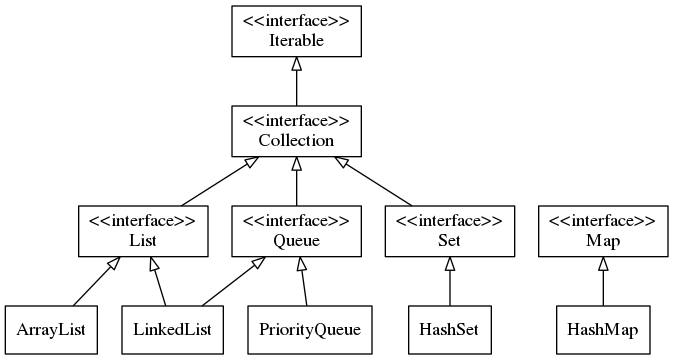
\includegraphics[width=0.9\textwidth]{java_util_overview_short}
\end{center}
}

